\PassOptionsToPackage{dvipsnames,table}{xcolor}
\documentclass[10pt]{beamer}
\usepackage{Cours}

\begin{document}


\newcounter{numchap}
\setcounter{numchap}{1}
\newcounter{numframe}
\setcounter{numframe}{0}
\newcommand{\mframe}[1]{\frametitle{#1} \addtocounter{numframe}{1}}
\newcommand{\cnum}{\fbox{\textcolor{yellow}{\textbf{C\thenumchap}}}~}
\newcommand{\makess}[1]{\section{#1} \label{ss\thesection}}
\newcommand{\stitle}{\textcolor{yellow}{\textbf{\thesection. \nameref{ss\thesection}}}}

\definecolor{codebg}{gray}{0.90}
\definecolor{grispale}{gray}{0.95}
\definecolor{fluo}{rgb}{1,0.96,0.62}
\newminted[langageC]{c}{linenos=true,escapeinside=||,highlightcolor=fluo,tabsize=2,breaklines=true}
\newminted[codepython]{python}{linenos=true,escapeinside=||,highlightcolor=fluo,tabsize=2,breaklines=true}
% Inclusion complète (ou partiel en indiquant premiere et dernière ligne) d'un fichier C
\newcommand{\inputC}[3]{\begin{mdframed}[backgroundcolor=codebg] \inputminted[breaklines=true,fontsize=#3,linenos=true,highlightcolor=fluo,tabsize=2,highlightlines={#2}]{c}{#1} \end{mdframed}}
\newcommand{\inputpartC}[5]{\begin{mdframed}[backgroundcolor=codebg] \inputminted[breaklines=true,fontsize=#3,linenos=true,highlightcolor=fluo,tabsize=2,highlightlines={#2},firstline=#4,lastline=#5,firstnumber=1]{c}{#1} \end{mdframed}}
\newcommand{\inputpython}[3]{\begin{mdframed}[backgroundcolor=codebg] \inputminted[breaklines=true,fontsize=#3,linenos=true,highlightcolor=fluo,tabsize=2,highlightlines={#2}]{python}{#1} \end{mdframed}}
\newcommand{\inputpartOCaml}[5]{\begin{mdframed}[backgroundcolor=codebg] \inputminted[breaklines=true,fontsize=#3,linenos=true,highlightcolor=fluo,tabsize=2,highlightlines={#2},firstline=#4,lastline=#5,firstnumber=1]{OCaml}{#1} \end{mdframed}}
\BeforeBeginEnvironment{minted}{\begin{mdframed}[backgroundcolor=codebg]}
\AfterEndEnvironment{minted}{\end{mdframed}}
\newcommand{\kw}[1]{\textcolor{blue}{\tt #1}}

\newtcolorbox{rcadre}[4]{halign=center,colback={#1},colframe={#2},width={#3cm},height={#4cm},valign=center,boxrule=1pt,left=0pt,right=0pt}
\newtcolorbox{cadre}[4]{halign=center,colback={#1},colframe={#2},arc=0mm,width={#3cm},height={#4cm},valign=center,boxrule=1pt,left=0pt,right=0pt}
\newcommand{\myem}[1]{\colorbox{fluo}{#1}}
\mdfsetup{skipabove=1pt,skipbelow=-2pt}



% Noeud dans un cadre pour les arbres
\newcommand{\noeud}[2]{\Tr{\fbox{\textcolor{#1}{\tt #2}}}}

\newcommand{\htmlmode}{\lstset{language=html,numbers=left, tabsize=4, frame=single, breaklines=true, keywordstyle=\ttfamily, basicstyle=\small,
   numberstyle=\tiny\ttfamily, framexleftmargin=0mm, backgroundcolor=\color{grispale}, xleftmargin=12mm,showstringspaces=false}}
\newcommand{\pythonmode}{\lstset{
   language=python,
   linewidth=\linewidth,
   numbers=left,
   tabsize=4,
   frame=single,
   breaklines=true,
   keywordstyle=\ttfamily\color{blue},
   basicstyle=\small,
   numberstyle=\tiny\ttfamily,
   framexleftmargin=-2mm,
   numbersep=-0.5mm,
   backgroundcolor=\color{codebg},
   xleftmargin=-1mm, 
   showstringspaces=false,
   commentstyle=\color{gray},
   stringstyle=\color{OliveGreen},
   emph={turtle,Screen,Turtle},
   emphstyle=\color{RawSienna},
   morekeywords={setheading,goto,backward,forward,left,right,pendown,penup,pensize,color,speed,hideturtle,showturtle,forward}}
   }
   \newcommand{\Cmode}{\lstset{
      language=[ANSI]C,
      linewidth=\linewidth,
      numbers=left,
      tabsize=4,
      frame=single,
      breaklines=true,
      keywordstyle=\ttfamily\color{blue},
      basicstyle=\small,
      numberstyle=\tiny\ttfamily,
      framexleftmargin=0mm,
      numbersep=2mm,
      backgroundcolor=\color{codebg},
      xleftmargin=0mm, 
      showstringspaces=false,
      commentstyle=\color{gray},
      stringstyle=\color{OliveGreen},
      emphstyle=\color{RawSienna},
      escapechar=\|,
      morekeywords={}}
      }
\newcommand{\bashmode}{\lstset{language=bash,numbers=left, tabsize=2, frame=single, breaklines=true, basicstyle=\ttfamily,
   numberstyle=\tiny\ttfamily, framexleftmargin=0mm, backgroundcolor=\color{grispale}, xleftmargin=12mm, showstringspaces=false}}
\newcommand{\exomode}{\lstset{language=python,numbers=left, tabsize=2, frame=single, breaklines=true, basicstyle=\ttfamily,
   numberstyle=\tiny\ttfamily, framexleftmargin=13mm, xleftmargin=12mm, basicstyle=\small, showstringspaces=false}}
   
   
  
%tei pour placer les images
%tei{nom de l’image}{échelle de l’image}{sens}{texte a positionner}
%sens ="1" (droite) ou "2" (gauche)
\newlength{\ltxt}
\newcommand{\tei}[4]{
\setlength{\ltxt}{\linewidth}
\setbox0=\hbox{\includegraphics[scale=#2]{#1}}
\addtolength{\ltxt}{-\wd0}
\addtolength{\ltxt}{-10pt}
\ifthenelse{\equal{#3}{1}}{
\begin{minipage}{\wd0}
\includegraphics[scale=#2]{#1}
\end{minipage}
\hfill
\begin{minipage}{\ltxt}
#4
\end{minipage}
}{
\begin{minipage}{\ltxt}
#4
\end{minipage}
\hfill
\begin{minipage}{\wd0}
\includegraphics[scale=#2]{#1}
\end{minipage}
}
}

%Juxtaposition d'une image pspciture et de texte 
%#1: = code pstricks de l'image
%#2: largeur de l'image
%#3: hauteur de l'image
%#4: Texte à écrire
\newcommand{\ptp}[4]{
\setlength{\ltxt}{\linewidth}
\addtolength{\ltxt}{-#2 cm}
\addtolength{\ltxt}{-0.1 cm}
\begin{minipage}[b][#3 cm][t]{\ltxt}
#4
\end{minipage}\hfill
\begin{minipage}[b][#3 cm][c]{#2 cm}
#1
\end{minipage}\par
}



%Macros pour les graphiques
\psset{linewidth=0.5\pslinewidth,PointSymbol=x}
\setlength{\fboxrule}{0.5pt}
\newcounter{tempangle}

%Marque la longueur du segment d'extrémité  #1 et  #2 avec la valeur #3, #4 est la distance par rapport au segment (en %age de la valeur de celui ci) et #5 l'orientation du marquage : +90 ou -90
\newcommand{\afflong}[5]{
\pstRotation[RotAngle=#4,PointSymbol=none,PointName=none]{#1}{#2}[X] 
\pstHomO[PointSymbol=none,PointName=none,HomCoef=#5]{#1}{X}[Y]
\pstTranslation[PointSymbol=none,PointName=none]{#1}{#2}{Y}[Z]
 \ncline{|<->|,linewidth=0.25\pslinewidth}{Y}{Z} \ncput*[nrot=:U]{\footnotesize{#3}}
}
\newcommand{\afflongb}[3]{
\ncline{|<->|,linewidth=0}{#1}{#2} \naput*[nrot=:U]{\footnotesize{#3}}
}

%Construis le point #4 situé à #2 cm du point #1 avant un angle #3 par rapport à l'horizontale. #5 = liste de paramètre
\newcommand{\lsegment}[5]{\pstGeonode[PointSymbol=none,PointName=none](0,0){O'}(#2,0){I'} \pstTranslation[PointSymbol=none,PointName=none]{O'}{I'}{#1}[J'] \pstRotation[RotAngle=#3,PointSymbol=x,#5]{#1}{J'}[#4]}
\newcommand{\tsegment}[5]{\pstGeonode[PointSymbol=none,PointName=none](0,0){O'}(#2,0){I'} \pstTranslation[PointSymbol=none,PointName=none]{O'}{I'}{#1}[J'] \pstRotation[RotAngle=#3,PointSymbol=x,#5]{#1}{J'}[#4] \pstLineAB{#4}{#1}}

%Construis le point #4 situé à #3 cm du point #1 et faisant un angle de  90° avec la droite (#1,#2) #5 = liste de paramètre
\newcommand{\psegment}[5]{
\pstGeonode[PointSymbol=none,PointName=none](0,0){O'}(#3,0){I'}
 \pstTranslation[PointSymbol=none,PointName=none]{O'}{I'}{#1}[J']
 \pstInterLC[PointSymbol=none,PointName=none]{#1}{#2}{#1}{J'}{M1}{M2} \pstRotation[RotAngle=-90,PointSymbol=x,#5]{#1}{M1}[#4]
  }
  
%Construis le point #4 situé à #3 cm du point #1 et faisant un angle de  #5° avec la droite (#1,#2) #6 = liste de paramètre
\newcommand{\mlogo}[6]{
\pstGeonode[PointSymbol=none,PointName=none](0,0){O'}(#3,0){I'}
 \pstTranslation[PointSymbol=none,PointName=none]{O'}{I'}{#1}[J']
 \pstInterLC[PointSymbol=none,PointName=none]{#1}{#2}{#1}{J'}{M1}{M2} \pstRotation[RotAngle=#5,PointSymbol=x,#6]{#1}{M2}[#4]
  }

% Construis un triangle avec #1=liste des 3 sommets séparés par des virgules, #2=liste des 3 longueurs séparés par des virgules, #3 et #4 : paramètre d'affichage des 2e et 3 points et #5 : inclinaison par rapport à l'horizontale
%autre macro identique mais sans tracer les segments joignant les sommets
\noexpandarg
\newcommand{\Triangleccc}[5]{
\StrBefore{#1}{,}[\pointA]
\StrBetween[1,2]{#1}{,}{,}[\pointB]
\StrBehind[2]{#1}{,}[\pointC]
\StrBefore{#2}{,}[\coteA]
\StrBetween[1,2]{#2}{,}{,}[\coteB]
\StrBehind[2]{#2}{,}[\coteC]
\tsegment{\pointA}{\coteA}{#5}{\pointB}{#3} 
\lsegment{\pointA}{\coteB}{0}{Z1}{PointSymbol=none, PointName=none}
\lsegment{\pointB}{\coteC}{0}{Z2}{PointSymbol=none, PointName=none}
\pstInterCC{\pointA}{Z1}{\pointB}{Z2}{\pointC}{Z3} 
\pstLineAB{\pointA}{\pointC} \pstLineAB{\pointB}{\pointC}
\pstSymO[PointName=\pointC,#4]{C}{C}[C]
}
\noexpandarg
\newcommand{\TrianglecccP}[5]{
\StrBefore{#1}{,}[\pointA]
\StrBetween[1,2]{#1}{,}{,}[\pointB]
\StrBehind[2]{#1}{,}[\pointC]
\StrBefore{#2}{,}[\coteA]
\StrBetween[1,2]{#2}{,}{,}[\coteB]
\StrBehind[2]{#2}{,}[\coteC]
\tsegment{\pointA}{\coteA}{#5}{\pointB}{#3} 
\lsegment{\pointA}{\coteB}{0}{Z1}{PointSymbol=none, PointName=none}
\lsegment{\pointB}{\coteC}{0}{Z2}{PointSymbol=none, PointName=none}
\pstInterCC[PointNameB=none,PointSymbolB=none,#4]{\pointA}{Z1}{\pointB}{Z2}{\pointC}{Z1} 
}


% Construis un triangle avec #1=liste des 3 sommets séparés par des virgules, #2=liste formée de 2 longueurs et d'un angle séparés par des virgules, #3 et #4 : paramètre d'affichage des 2e et 3 points et #5 : inclinaison par rapport à l'horizontale
%autre macro identique mais sans tracer les segments joignant les sommets
\newcommand{\Trianglecca}[5]{
\StrBefore{#1}{,}[\pointA]
\StrBetween[1,2]{#1}{,}{,}[\pointB]
\StrBehind[2]{#1}{,}[\pointC]
\StrBefore{#2}{,}[\coteA]
\StrBetween[1,2]{#2}{,}{,}[\coteB]
\StrBehind[2]{#2}{,}[\angleA]
\tsegment{\pointA}{\coteA}{#5}{\pointB}{#3} 
\setcounter{tempangle}{#5}
\addtocounter{tempangle}{\angleA}
\tsegment{\pointA}{\coteB}{\thetempangle}{\pointC}{#4}
\pstLineAB{\pointB}{\pointC}
}
\newcommand{\TriangleccaP}[5]{
\StrBefore{#1}{,}[\pointA]
\StrBetween[1,2]{#1}{,}{,}[\pointB]
\StrBehind[2]{#1}{,}[\pointC]
\StrBefore{#2}{,}[\coteA]
\StrBetween[1,2]{#2}{,}{,}[\coteB]
\StrBehind[2]{#2}{,}[\angleA]
\lsegment{\pointA}{\coteA}{#5}{\pointB}{#3} 
\setcounter{tempangle}{#5}
\addtocounter{tempangle}{\angleA}
\lsegment{\pointA}{\coteB}{\thetempangle}{\pointC}{#4}
}

% Construis un triangle avec #1=liste des 3 sommets séparés par des virgules, #2=liste formée de 1 longueurs et de deux angle séparés par des virgules, #3 et #4 : paramètre d'affichage des 2e et 3 points et #5 : inclinaison par rapport à l'horizontale
%autre macro identique mais sans tracer les segments joignant les sommets
\newcommand{\Trianglecaa}[5]{
\StrBefore{#1}{,}[\pointA]
\StrBetween[1,2]{#1}{,}{,}[\pointB]
\StrBehind[2]{#1}{,}[\pointC]
\StrBefore{#2}{,}[\coteA]
\StrBetween[1,2]{#2}{,}{,}[\angleA]
\StrBehind[2]{#2}{,}[\angleB]
\tsegment{\pointA}{\coteA}{#5}{\pointB}{#3} 
\setcounter{tempangle}{#5}
\addtocounter{tempangle}{\angleA}
\lsegment{\pointA}{1}{\thetempangle}{Z1}{PointSymbol=none, PointName=none}
\setcounter{tempangle}{#5}
\addtocounter{tempangle}{180}
\addtocounter{tempangle}{-\angleB}
\lsegment{\pointB}{1}{\thetempangle}{Z2}{PointSymbol=none, PointName=none}
\pstInterLL[#4]{\pointA}{Z1}{\pointB}{Z2}{\pointC}
\pstLineAB{\pointA}{\pointC}
\pstLineAB{\pointB}{\pointC}
}
\newcommand{\TrianglecaaP}[5]{
\StrBefore{#1}{,}[\pointA]
\StrBetween[1,2]{#1}{,}{,}[\pointB]
\StrBehind[2]{#1}{,}[\pointC]
\StrBefore{#2}{,}[\coteA]
\StrBetween[1,2]{#2}{,}{,}[\angleA]
\StrBehind[2]{#2}{,}[\angleB]
\lsegment{\pointA}{\coteA}{#5}{\pointB}{#3} 
\setcounter{tempangle}{#5}
\addtocounter{tempangle}{\angleA}
\lsegment{\pointA}{1}{\thetempangle}{Z1}{PointSymbol=none, PointName=none}
\setcounter{tempangle}{#5}
\addtocounter{tempangle}{180}
\addtocounter{tempangle}{-\angleB}
\lsegment{\pointB}{1}{\thetempangle}{Z2}{PointSymbol=none, PointName=none}
\pstInterLL[#4]{\pointA}{Z1}{\pointB}{Z2}{\pointC}
}

%Construction d'un cercle de centre #1 et de rayon #2 (en cm)
\newcommand{\Cercle}[2]{
\lsegment{#1}{#2}{0}{Z1}{PointSymbol=none, PointName=none}
\pstCircleOA{#1}{Z1}
}

%construction d'un parallélogramme #1 = liste des sommets, #2 = liste contenant les longueurs de 2 côtés consécutifs et leurs angles;  #3, #4 et #5 : paramètre d'affichage des sommets #6 inclinaison par rapport à l'horizontale 
% meme macro sans le tracé des segements
\newcommand{\Para}[6]{
\StrBefore{#1}{,}[\pointA]
\StrBetween[1,2]{#1}{,}{,}[\pointB]
\StrBetween[2,3]{#1}{,}{,}[\pointC]
\StrBehind[3]{#1}{,}[\pointD]
\StrBefore{#2}{,}[\longueur]
\StrBetween[1,2]{#2}{,}{,}[\largeur]
\StrBehind[2]{#2}{,}[\angle]
\tsegment{\pointA}{\longueur}{#6}{\pointB}{#3} 
\setcounter{tempangle}{#6}
\addtocounter{tempangle}{\angle}
\tsegment{\pointA}{\largeur}{\thetempangle}{\pointD}{#5}
\pstMiddleAB[PointName=none,PointSymbol=none]{\pointB}{\pointD}{Z1}
\pstSymO[#4]{Z1}{\pointA}[\pointC]
\pstLineAB{\pointB}{\pointC}
\pstLineAB{\pointC}{\pointD}
}
\newcommand{\ParaP}[6]{
\StrBefore{#1}{,}[\pointA]
\StrBetween[1,2]{#1}{,}{,}[\pointB]
\StrBetween[2,3]{#1}{,}{,}[\pointC]
\StrBehind[3]{#1}{,}[\pointD]
\StrBefore{#2}{,}[\longueur]
\StrBetween[1,2]{#2}{,}{,}[\largeur]
\StrBehind[2]{#2}{,}[\angle]
\lsegment{\pointA}{\longueur}{#6}{\pointB}{#3} 
\setcounter{tempangle}{#6}
\addtocounter{tempangle}{\angle}
\lsegment{\pointA}{\largeur}{\thetempangle}{\pointD}{#5}
\pstMiddleAB[PointName=none,PointSymbol=none]{\pointB}{\pointD}{Z1}
\pstSymO[#4]{Z1}{\pointA}[\pointC]
}


%construction d'un cerf-volant #1 = liste des sommets, #2 = liste contenant les longueurs de 2 côtés consécutifs et leurs angles;  #3, #4 et #5 : paramètre d'affichage des sommets #6 inclinaison par rapport à l'horizontale 
% meme macro sans le tracé des segements
\newcommand{\CerfVolant}[6]{
\StrBefore{#1}{,}[\pointA]
\StrBetween[1,2]{#1}{,}{,}[\pointB]
\StrBetween[2,3]{#1}{,}{,}[\pointC]
\StrBehind[3]{#1}{,}[\pointD]
\StrBefore{#2}{,}[\longueur]
\StrBetween[1,2]{#2}{,}{,}[\largeur]
\StrBehind[2]{#2}{,}[\angle]
\tsegment{\pointA}{\longueur}{#6}{\pointB}{#3} 
\setcounter{tempangle}{#6}
\addtocounter{tempangle}{\angle}
\tsegment{\pointA}{\largeur}{\thetempangle}{\pointD}{#5}
\pstOrtSym[#4]{\pointB}{\pointD}{\pointA}[\pointC]
\pstLineAB{\pointB}{\pointC}
\pstLineAB{\pointC}{\pointD}
}

%construction d'un quadrilatère quelconque #1 = liste des sommets, #2 = liste contenant les longueurs des 4 côtés et l'angle entre 2 cotés consécutifs  #3, #4 et #5 : paramètre d'affichage des sommets #6 inclinaison par rapport à l'horizontale 
% meme macro sans le tracé des segements
\newcommand{\Quadri}[6]{
\StrBefore{#1}{,}[\pointA]
\StrBetween[1,2]{#1}{,}{,}[\pointB]
\StrBetween[2,3]{#1}{,}{,}[\pointC]
\StrBehind[3]{#1}{,}[\pointD]
\StrBefore{#2}{,}[\coteA]
\StrBetween[1,2]{#2}{,}{,}[\coteB]
\StrBetween[2,3]{#2}{,}{,}[\coteC]
\StrBetween[3,4]{#2}{,}{,}[\coteD]
\StrBehind[4]{#2}{,}[\angle]
\tsegment{\pointA}{\coteA}{#6}{\pointB}{#3} 
\setcounter{tempangle}{#6}
\addtocounter{tempangle}{\angle}
\tsegment{\pointA}{\coteD}{\thetempangle}{\pointD}{#5}
\lsegment{\pointB}{\coteB}{0}{Z1}{PointSymbol=none, PointName=none}
\lsegment{\pointD}{\coteC}{0}{Z2}{PointSymbol=none, PointName=none}
\pstInterCC[PointNameA=none,PointSymbolA=none,#4]{\pointB}{Z1}{\pointD}{Z2}{Z3}{\pointC} 
\pstLineAB{\pointB}{\pointC}
\pstLineAB{\pointC}{\pointD}
}


% Définition des colonnes centrées ou à droite pour tabularx
\newcolumntype{Y}{>{\centering\arraybackslash}X}
\newcolumntype{Z}{>{\flushright\arraybackslash}X}

%Les pointillés à remplir par les élèves
\newcommand{\po}[1]{\makebox[#1 cm]{\dotfill}}
\newcommand{\lpo}[1][3]{%
\multido{}{#1}{\makebox[\linewidth]{\dotfill}
}}

%Liste des pictogrammes utilisés sur la fiche d'exercice ou d'activités
\newcommand{\bombe}{\faBomb}
\newcommand{\livre}{\faBook}
\newcommand{\calculatrice}{\faCalculator}
\newcommand{\oral}{\faCommentO}
\newcommand{\surfeuille}{\faEdit}
\newcommand{\ordinateur}{\faLaptop}
\newcommand{\ordi}{\faDesktop}
\newcommand{\ciseaux}{\faScissors}
\newcommand{\danger}{\faExclamationTriangle}
\newcommand{\out}{\faSignOut}
\newcommand{\cadeau}{\faGift}
\newcommand{\flash}{\faBolt}
\newcommand{\lumiere}{\faLightbulb}
\newcommand{\compas}{\dsmathematical}
\newcommand{\calcullitteral}{\faTimesCircleO}
\newcommand{\raisonnement}{\faCogs}
\newcommand{\recherche}{\faSearch}
\newcommand{\rappel}{\faHistory}
\newcommand{\video}{\faFilm}
\newcommand{\capacite}{\faPuzzlePiece}
\newcommand{\aide}{\faLifeRing}
\newcommand{\loin}{\faExternalLink}
\newcommand{\groupe}{\faUsers}
\newcommand{\bac}{\faGraduationCap}
\newcommand{\histoire}{\faUniversity}
\newcommand{\coeur}{\faSave}
\newcommand{\python}{\faPython}
\newcommand{\os}{\faMicrochip}
\newcommand{\rd}{\faCubes}
\newcommand{\data}{\faColumns}
\newcommand{\web}{\faCode}
\newcommand{\prog}{\faFile}
\newcommand{\algo}{\faCogs}
\newcommand{\important}{\faExclamationCircle}
\newcommand{\maths}{\faTimesCircle}
% Traitement des données en tables
\newcommand{\tables}{\faColumns}
% Types construits
\newcommand{\construits}{\faCubes}
% Type et valeurs de base
\newcommand{\debase}{{\footnotesize \faCube}}
% Systèmes d'exploitation
\newcommand{\linux}{\faLinux}
\newcommand{\sd}{\faProjectDiagram}
\newcommand{\bd}{\faDatabase}

%Les ensembles de nombres
\renewcommand{\N}{\mathbb{N}}
\newcommand{\D}{\mathbb{D}}
\newcommand{\Z}{\mathbb{Z}}
\newcommand{\Q}{\mathbb{Q}}
\newcommand{\R}{\mathbb{R}}
\newcommand{\C}{\mathbb{C}}

%Ecriture des vecteurs
\newcommand{\vect}[1]{\vbox{\halign{##\cr 
  \tiny\rightarrowfill\cr\noalign{\nointerlineskip\vskip1pt} 
  $#1\mskip2mu$\cr}}}


%Compteur activités/exos et question et mise en forme titre et questions
\newcounter{numact}
\setcounter{numact}{1}
\newcounter{numseance}
\setcounter{numseance}{1}
\newcounter{numexo}
\setcounter{numexo}{0}
\newcounter{numprojet}
\setcounter{numprojet}{0}
\newcounter{numquestion}
\newcommand{\espace}[1]{\rule[-1ex]{0pt}{#1 cm}}
\newcommand{\Quest}[3]{
\addtocounter{numquestion}{1}
\begin{tabularx}{\textwidth}{X|m{1cm}|}
\cline{2-2}
\textbf{\sffamily{\alph{numquestion})}} #1 & \dots / #2 \\
\hline 
\multicolumn{2}{|l|}{\espace{#3}} \\
\hline
\end{tabularx}
}
\newcommand{\QuestR}[3]{
\addtocounter{numquestion}{1}
\begin{tabularx}{\textwidth}{X|m{1cm}|}
\cline{2-2}
\textbf{\sffamily{\alph{numquestion})}} #1 & \dots / #2 \\
\hline 
\multicolumn{2}{|l|}{\cor{#3}} \\
\hline
\end{tabularx}
}
\newcommand{\Pre}{{\sc nsi} 1\textsuperscript{e}}
\newcommand{\Term}{{\sc nsi} Terminale}
\newcommand{\Sec}{2\textsuperscript{e}}
\newcommand{\Exo}[2]{ \addtocounter{numexo}{1} \ding{113} \textbf{\sffamily{Exercice \thenumexo}} : \textit{#1} \hfill #2  \setcounter{numquestion}{0}}
\newcommand{\Projet}[1]{ \addtocounter{numprojet}{1} \ding{118} \textbf{\sffamily{Projet \thenumprojet}} : \textit{#1}}
\newcommand{\ExoD}[2]{ \addtocounter{numexo}{1} \ding{113} \textbf{\sffamily{Exercice \thenumexo}}  \textit{(#1 pts)} \hfill #2  \setcounter{numquestion}{0}}
\newcommand{\ExoB}[2]{ \addtocounter{numexo}{1} \ding{113} \textbf{\sffamily{Exercice \thenumexo}}  \textit{(Bonus de +#1 pts maximum)} \hfill #2  \setcounter{numquestion}{0}}
\newcommand{\Act}[2]{ \ding{113} \textbf{\sffamily{Activité \thenumact}} : \textit{#1} \hfill #2  \addtocounter{numact}{1} \setcounter{numquestion}{0}}
\newcommand{\Seance}{ \rule{1.5cm}{0.5pt}\raisebox{-3pt}{\framebox[4cm]{\textbf{\sffamily{Séance \thenumseance}}}}\hrulefill  \\
  \addtocounter{numseance}{1}}
\newcommand{\Acti}[2]{ {\footnotesize \ding{117}} \textbf{\sffamily{Activité \thenumact}} : \textit{#1} \hfill #2  \addtocounter{numact}{1} \setcounter{numquestion}{0}}
\newcommand{\titre}[1]{\begin{Large}\textbf{\ding{118}}\end{Large} \begin{large}\textbf{ #1}\end{large} \vspace{0.2cm}}
\newcommand{\QListe}[1][0]{
\ifthenelse{#1=0}
{\begin{enumerate}[partopsep=0pt,topsep=0pt,parsep=0pt,itemsep=0pt,label=\textbf{\sffamily{\arabic*.}},series=question]}
{\begin{enumerate}[resume*=question]}}
\newcommand{\SQListe}[1][0]{
\ifthenelse{#1=0}
{\begin{enumerate}[partopsep=0pt,topsep=0pt,parsep=0pt,itemsep=0pt,label=\textbf{\sffamily{\alph*)}},series=squestion]}
{\begin{enumerate}[resume*=squestion]}}
\newcommand{\SQListeL}[1][0]{
\ifthenelse{#1=0}
{\begin{enumerate*}[partopsep=0pt,topsep=0pt,parsep=0pt,itemsep=0pt,label=\textbf{\sffamily{\alph*)}},series=squestion]}
{\begin{enumerate*}[resume*=squestion]}}
\newcommand{\FinListe}{\end{enumerate}}
\newcommand{\FinListeL}{\end{enumerate*}}

%Mise en forme de la correction
\newcommand{\cor}[1]{\par \textcolor{OliveGreen}{#1}}
\newcommand{\br}[1]{\cor{\textbf{#1}}}
\newcommand{\tcor}[1]{\begin{tcolorbox}[width=0.92\textwidth,colback={white},colbacktitle=white,coltitle=OliveGreen,colframe=green!75!black,boxrule=0.2mm]   
\cor{#1}
\end{tcolorbox}
}
\newcommand{\rc}[1]{\textcolor{OliveGreen}{#1}}
\newcommand{\pmc}[1]{\textcolor{blue}{\tt #1}}
\newcommand{\tmc}[1]{\textcolor{RawSienna}{\tt #1}}


%Référence aux exercices par leur numéro
\newcommand{\refexo}[1]{
\refstepcounter{numexo}
\addtocounter{numexo}{-1}
\label{#1}}

%Séparation entre deux activités
\newcommand{\separateur}{\begin{center}
\rule{1.5cm}{0.5pt}\raisebox{-3pt}{\ding{117}}\rule{1.5cm}{0.5pt}  \vspace{0.2cm}
\end{center}}

%Entête et pied de page
\newcommand{\snt}[1]{\lhead{\textbf{SNT -- La photographie numérique} \rhead{\textit{Lycée Nord}}}}
\newcommand{\Activites}[2]{\lhead{\textbf{{\sc #1}}}
\rhead{Activités -- \textbf{#2}}
\cfoot{}}
\newcommand{\Exos}[2]{\lhead{\textbf{Fiche d'exercices: {\sc #1}}}
\rhead{Niveau: \textbf{#2}}
\cfoot{}}
\newcommand{\Devoir}[2]{\lhead{\textbf{Devoir de mathématiques : {\sc #1}}}
\rhead{\textbf{#2}} \setlength{\fboxsep}{8pt}
\begin{center}
%Titre de la fiche
\fbox{\parbox[b][1cm][t]{0.3\textwidth}{Nom : \hfill \po{3} \par \vfill Prénom : \hfill \po{3}} } \hfill 
\fbox{\parbox[b][1cm][t]{0.6\textwidth}{Note : \po{1} / 20} }
\end{center} \cfoot{}}

%Devoir programmation en NSI (pas à rendre sur papier)
\newcommand{\PNSI}[2]{\lhead{\textbf{Devoir de {\sc nsi} : \textsf{ #1}}}
\rhead{\textbf{#2}} \setlength{\fboxsep}{8pt}
\begin{tcolorbox}[title=\textcolor{black}{\danger\; A lire attentivement},colbacktitle=lightgray]
{\begin{enumerate}
\item Rendre tous vous programmes en les envoyant par mail à l'adresse {\tt fnativel2@ac-reunion.fr}, en précisant bien dans le sujet vos noms et prénoms
\item Un programme qui fonctionne mal ou pas du tout peut rapporter des points
\item Les bonnes pratiques de programmation (clarté et lisiblité du code) rapportent des points
\end{enumerate}
}
\end{tcolorbox}
 \cfoot{}}


%Devoir de NSI
\newcommand{\DNSI}[2]{\lhead{\textbf{Devoir de {\sc nsi} : \textsf{ #1}}}
\rhead{\textbf{#2}} \setlength{\fboxsep}{8pt}
\begin{center}
%Titre de la fiche
\fbox{\parbox[b][1cm][t]{0.3\textwidth}{Nom : \hfill \po{3} \par \vfill Prénom : \hfill \po{3}} } \hfill 
\fbox{\parbox[b][1cm][t]{0.6\textwidth}{Note : \po{1} / 10} }
\end{center} \cfoot{}}

\newcommand{\DevoirNSI}[2]{\lhead{\textbf{Devoir de {\sc nsi} : {\sc #1}}}
\rhead{\textbf{#2}} \setlength{\fboxsep}{8pt}
\cfoot{}}

%La définition de la commande QCM pour auto-multiple-choice
%En premier argument le sujet du qcm, deuxième argument : la classe, 3e : la durée prévue et #4 : présence ou non de questions avec plusieurs bonnes réponses
\newcommand{\QCM}[4]{
{\large \textbf{\ding{52} QCM : #1}} -- Durée : \textbf{#3 min} \hfill {\large Note : \dots/10} 
\hrule \vspace{0.1cm}\namefield{}
Nom :  \textbf{\textbf{\nom{}}} \qquad \qquad Prénom :  \textbf{\prenom{}}  \hfill Classe: \textbf{#2}
\vspace{0.2cm}
\hrule  
\begin{itemize}[itemsep=0pt]
\item[-] \textit{Une bonne réponse vaut un point, une absence de réponse n'enlève pas de point. }
\item[\danger] \textit{Une mauvaise réponse enlève un point.}
\ifthenelse{#4=1}{\item[-] \textit{Les questions marquées du symbole \multiSymbole{} peuvent avoir plusieurs bonnes réponses possibles.}}{}
\end{itemize}
}
\newcommand{\DevoirC}[2]{
\renewcommand{\footrulewidth}{0.5pt}
\lhead{\textbf{Devoir de mathématiques : {\sc #1}}}
\rhead{\textbf{#2}} \setlength{\fboxsep}{8pt}
\fbox{\parbox[b][0.4cm][t]{0.955\textwidth}{Nom : \po{5} \hfill Prénom : \po{5} \hfill Classe: \textbf{1}\textsuperscript{$\dots$}} } 
\rfoot{\thepage} \cfoot{} \lfoot{Lycée Nord}}
\newcommand{\DevoirInfo}[2]{\lhead{\textbf{Evaluation : {\sc #1}}}
\rhead{\textbf{#2}} \setlength{\fboxsep}{8pt}
 \cfoot{}}
\newcommand{\DM}[2]{\lhead{\textbf{Devoir maison à rendre le #1}} \rhead{\textbf{#2}}}

%Macros permettant l'affichage des touches de la calculatrice
%Touches classiques : #1 = 0 fond blanc pour les nombres et #1= 1gris pour les opérations et entrer, second paramètre=contenu
%Si #2=1 touche arrondi avec fond gris
\newcommand{\TCalc}[2]{
\setlength{\fboxsep}{0.1pt}
\ifthenelse{#1=0}
{\psframebox[fillstyle=solid, fillcolor=white]{\parbox[c][0.25cm][c]{0.6cm}{\centering #2}}}
{\ifthenelse{#1=1}
{\psframebox[fillstyle=solid, fillcolor=lightgray]{\parbox[c][0.25cm][c]{0.6cm}{\centering #2}}}
{\psframebox[framearc=.5,fillstyle=solid, fillcolor=white]{\parbox[c][0.25cm][c]{0.6cm}{\centering #2}}}
}}
\newcommand{\Talpha}{\psdblframebox[fillstyle=solid, fillcolor=white]{\hspace{-0.05cm}\parbox[c][0.25cm][c]{0.65cm}{\centering \scriptsize{alpha}}} \;}
\newcommand{\Tsec}{\psdblframebox[fillstyle=solid, fillcolor=white]{\parbox[c][0.25cm][c]{0.6cm}{\centering \scriptsize 2nde}} \;}
\newcommand{\Tfx}{\psdblframebox[fillstyle=solid, fillcolor=white]{\parbox[c][0.25cm][c]{0.6cm}{\centering \scriptsize $f(x)$}} \;}
\newcommand{\Tvar}{\psframebox[framearc=.5,fillstyle=solid, fillcolor=white]{\hspace{-0.22cm} \parbox[c][0.25cm][c]{0.82cm}{$\scriptscriptstyle{X,T,\theta,n}$}}}
\newcommand{\Tgraphe}{\psdblframebox[fillstyle=solid, fillcolor=white]{\hspace{-0.08cm}\parbox[c][0.25cm][c]{0.68cm}{\centering \tiny{graphe}}} \;}
\newcommand{\Tfen}{\psdblframebox[fillstyle=solid, fillcolor=white]{\hspace{-0.08cm}\parbox[c][0.25cm][c]{0.68cm}{\centering \tiny{fenêtre}}} \;}
\newcommand{\Ttrace}{\psdblframebox[fillstyle=solid, fillcolor=white]{\parbox[c][0.25cm][c]{0.6cm}{\centering \scriptsize{trace}}} \;}

% Macroi pour l'affichage  d'un entier n dans  une base b
\newcommand{\base}[2]{ \overline{#1}^{#2}}
% Intervalle d'entiers
\newcommand{\intN}[2]{\llbracket #1; #2 \rrbracket}}

% Numéro et titre de chapitre
\setcounter{numchap}{13}
\newcommand{\Ctitle}{\cnum {Force brute, retour sur trace}}
\newcommand{\SPATH}{/home/fenarius/Travail/Cours/cpge-info/docs/mp2i/files/C\thenumchap/}

\makess{Force brute : généralités}
\begin{frame}[fragile]{\Ctitle}{\stitle}
	\begin{alertblock}{Définition}
		La recherche par \textcolor{blue}{force brute} (\textit{brute force}) consiste à parcourir toutes les solutions possibles d'un problème en testant si elles conviennent.\\
		\onslide<2->{De façon formelle, si on note $V$ l'ensemble des candidats, et $P$ une propriété des éléments de $V$, on teste (en les énumérant) les $x \in V$ jusqu'à en trouver un qui vérifie $P$.}
	\end{alertblock}
	\onslide<3->{
		\begin{block}{Remarques}
			\begin{itemize}
				\item<3-> Dans certains problèmes on cherche à déterminer \textit{toutes} les solutions et donc on ne s'arrête pas à la première rencontrée
				\item<4-> On doit pouvoir \textcolor{blue}{énumérer de façon exhaustive} les éléments de $V$ (ce qui peut être difficile dans certains cas).
			\end{itemize}
		\end{block}}
\end{frame}

\begin{frame}[fragile]{\Ctitle}{\stitle}
	\begin{exampleblock}{Exemple}
		\begin{itemize}
			\item La recherche d'un mot de passe par force brute : $V$ est l'ensemble des chaines de caractères et $P(x)$ est vérifié si $x$ est le mot de passe cherché. Dans ce cas on pourra réaliser l'énumération des candidats en commençant par les chaines de longueur 1, puis 2, \dots
			\item<2-> $V$ est l'ensemble des grilles complétées d'un sudoku et $P$ vérifie si la grille est valide.
			\item<3-> $V$ est l'ensemble des permutations possibles d'une liste d'entiers et $P$ vérifie si la permutation est triée en ordre croissant (\textcolor{blue}{bogosort}).
		\end{itemize}
	\end{exampleblock}
\end{frame}

\begin{frame}[fragile]{\Ctitle}{\stitle}
	\begin{block}{Complexité}
		En supposant l'ensemble $V$ fini, une recherche exhaustive effectue au plus $|V|$ itérations.\\
		\textcolor{BrickRed}{\small \danger} Cela ne signifie pas que la complexité est toujours en $O(V)$ car tester si une solution vérifie $P$ ou non peut avoir un coût non constant.
	\end{block}
	\begin{block}{Problème d'optimisation}
		Dans les problèmes du type \og{} \textit{déterminer $x \in V$ tel que $f(x)$ soit minimale (ou maximale)} \fg{}, l'exploration exhaustive va résoudre le problème en calculant toutes les images par $f$ des éléments de V.
	\end{block}
\end{frame}

\makess{Mot de passe par force brute}
\begin{frame}[fragile]{\Ctitle}{\stitle}
	\begin{exampleblock}{Exercice}
		Tableau des temps pour la recherche de mot de passe par force brute :
		\begin{center}
			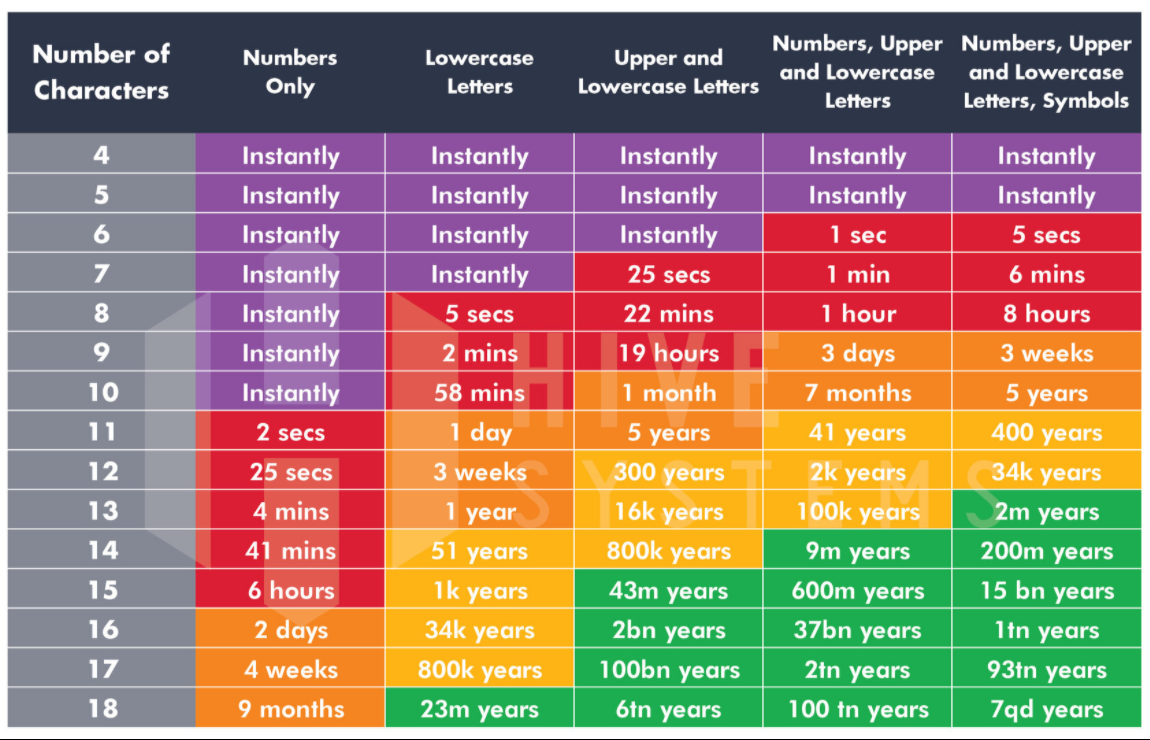
\includegraphics[width=130px]{mdp.eps}
		\end{center}
		On s'intéresse à la recherche d'un mot de passe de 8 lettres minusucles.
		\begin{itemize}
			\item<2-> Combien il y a-t-il de mots de passes possibles ? Quel est le temps indiqué dans le tableau ?
			\item<3-> Proposer un algorithme permettant d'énumérer les possibilités.
			\item<4-> Ecrire en C, une fonction de signature \mintinline{c}{char *bruteforce(char *mdp, char *charset, int size)
				} qui implémente une recherche de mot de passe par force brute.
		\end{itemize}
	\end{exampleblock}
\end{frame}

\begin{frame}[fragile]{\Ctitle}{\stitle}
	\begin{exampleblock}{Proposition de solution}
		\inputpartC{\SPATH/mdp.c}{}{\tiny}{5}{35}
	\end{exampleblock}
\end{frame}

\makess{Résolution par retour sur trace}
\begin{frame}[fragile]{\Ctitle}{\stitle}
	\begin{alertblock}{Définition}
		Le \textcolor{blue}{retour sur trace} (\textit{backtracking}) consiste à construire la solution d'un problème à partir d'une solution partielle. On s'arrête dès qu'une incohérence est rencontrée dans la solution partielle et on revient en arrière afin de modifier une décision prise précédemment.
	\end{alertblock}
	\onslide<2->{
		\begin{exampleblock}{Exemple}
			Pour résoudre un Sudoku :
			\begin{itemize}
				\item<3-> La force brute parcourt l'ensemble des valeurs possibles pour toutes les cases restantes
				\item<4-> Le \textit{backtracking} place des valeurs au fur et à mesure et revient en arrière si une impossibilité est rencontrée.
			\end{itemize}
		\end{exampleblock}}
\end{frame}

\makess{Résolution du problème des n reines par \textit{backtracking}}
\newcommand{\queen}{\textcolor{BrickRed}{\!\faChessQueen}}
\begin{frame}[fragile]{\Ctitle}{\stitle}
	\begin{exampleblock}{Exemple}
		{\small Le problème des $n$ reines consiste à placer $n$ reines sur une échiquier de taille $n$ de façon à ce deux reines ne soit pas sur la même ligne, même colonne ou même colonne (c'est à dire qu'aucune reine n'en menace une autre) \\}
		\smallskip
		\onslide<2->{\small Une solution dans le cas $n=8$ est proposée ci-dessous :
			\begin{center}
				\input{\SPATH/sol42}
			\end{center}}
	\end{exampleblock}
\end{frame}


\begin{frame}[fragile]{\Ctitle}{\stitle}
	\begin{exampleblock}{Représentation du problème}
        \begin{itemize}
		\item <1-> On sait qu'il y a une seule reine par colonne, on peut donc représenter une position de jeu par un tableau de taille $n$ contenant les numéros de ligne des $k$ reines déjà placées.
		\item <2-> L'algorithme va alors consister à tenter de placer la reine $k+1$ sur chacune des lignes $0, \dots, k-1$
		\begin{itemize}
            \item si cela génère une menace, on essayer la possibilité suivante, en revenant récursivement à la reine précédente si nécesssaire
            \item sinon on place la reine suivante, si c'est la dernière reine, une solution est trouvée.
        \end{itemize}
    \end{itemize}
	\end{exampleblock}
\end{frame}

\begin{frame}[fragile]{\Ctitle}{\stitle}
	\begin{exampleblock}{Début de l'algorithme ($n=4$)}
        \begin{tabularx}{\textwidth}{YYY}
            \renewcommand{\arraystretch}{1.5}
 \begin{tabular}{|P{0.2cm}|P{0.2cm}|P{0.2cm}|P{0.2cm}|P{0.2cm}|P{0.2cm}|P{0.2cm}|P{0.2cm}|} 
 \hline\cellcolor{white}{}&\cellcolor{black!30}{}&\cellcolor{white}{}&\cellcolor{black!30}{}\\
 \hline 
\cellcolor{black!30}{}&\cellcolor{white}{}&\cellcolor{black!30}{}&\cellcolor{white}{}\\
 \hline 
\cellcolor{white}{}&\cellcolor{black!30}{}&\cellcolor{white}{}&\cellcolor{black!30}{}\\
 \hline 
\cellcolor{black!30}{\queen}&\cellcolor{white}{}&\cellcolor{black!30}{}&\cellcolor{white}{}\\
 \hline 
\end{tabular}  & \leavevmode{\onslide<2->{\renewcommand{\arraystretch}{1.5}\begin{tabular}{|P{0.2cm}|P{0.2cm}|P{0.2cm}|P{0.2cm}|P{0.2cm}|P{0.2cm}|P{0.2cm}|P{0.2cm}|} 
    \hline\cellcolor{white}{}&\cellcolor{black!30}{}&\cellcolor{white}{}&\cellcolor{black!30}{}\\
    \hline 
   \cellcolor{black!30}{}&\cellcolor{white}{}&\cellcolor{black!30}{}&\cellcolor{white}{}\\
    \hline 
   \cellcolor{white}{}&\cellcolor{black!30}{}&\cellcolor{white}{}&\cellcolor{black!30}{}\\
    \hline 
   \cellcolor{black!30}{\queen}&\cellcolor{white}{\queen}&\cellcolor{black!30}{}&\cellcolor{white}{}\\
    \hline 
   \end{tabular}}} &
   \leavevmode{\onslide<3->{\renewcommand{\arraystretch}{1.5}\begin{tabular}{|P{0.2cm}|P{0.2cm}|P{0.2cm}|P{0.2cm}|P{0.2cm}|P{0.2cm}|P{0.2cm}|P{0.2cm}|} 
    \hline\cellcolor{white}{}&\cellcolor{black!30}{}&\cellcolor{white}{}&\cellcolor{black!30}{}\\
    \hline 
   \cellcolor{black!30}{}&\cellcolor{white}{}&\cellcolor{black!30}{}&\cellcolor{white}{}\\
    \hline 
   \cellcolor{white}{}&\cellcolor{black!30}{\queen}&\cellcolor{white}{}&\cellcolor{black!30}{}\\
    \hline 
   \cellcolor{black!30}{\queen}&\cellcolor{white}{}&\cellcolor{black!30}{}&\cellcolor{white}{}\\
    \hline 
   \end{tabular}}}\\
   & & \\
   \leavevmode{\onslide<4->{\renewcommand{\arraystretch}{1.5}\begin{tabular}{|P{0.2cm}|P{0.2cm}|P{0.2cm}|P{0.2cm}|P{0.2cm}|P{0.2cm}|P{0.2cm}|P{0.2cm}|} 
    \hline\cellcolor{white}{}&\cellcolor{black!30}{}&\cellcolor{white}{}&\cellcolor{black!30}{}\\
    \hline 
   \cellcolor{black!30}{}&\cellcolor{white}{\queen}&\cellcolor{black!30}{}&\cellcolor{white}{}\\
    \hline 
   \cellcolor{white}{}&\cellcolor{black!30}{}&\cellcolor{white}{}&\cellcolor{black!30}{}\\
    \hline 
   \cellcolor{black!30}{\queen}&\cellcolor{white}{}&\cellcolor{black!30}{}&\cellcolor{white}{}\\
    \hline 
   \end{tabular}}} & 
   \leavevmode{\onslide<5->{\renewcommand{\arraystretch}{1.5}\begin{tabular}{|P{0.2cm}|P{0.2cm}|P{0.2cm}|P{0.2cm}|P{0.2cm}|P{0.2cm}|P{0.2cm}|P{0.2cm}|} 
    \hline\cellcolor{white}{}&\cellcolor{black!30}{}&\cellcolor{white}{}&\cellcolor{black!30}{}\\
    \hline 
   \cellcolor{black!30}{}&\cellcolor{white}{\queen}&\cellcolor{black!30}{}&\cellcolor{white}{}\\
    \hline 
   \cellcolor{white}{}&\cellcolor{black!30}{}&\cellcolor{white}{}&\cellcolor{black!30}{}\\
    \hline 
   \cellcolor{black!30}{\queen}&\cellcolor{white}{}&\cellcolor{black!30}{\queen}&\cellcolor{white}{}\\
    \hline 
   \end{tabular}}}
   & 
   \leavevmode{\onslide<6->{\renewcommand{\arraystretch}{1.5}\begin{tabular}{|P{0.2cm}|P{0.2cm}|P{0.2cm}|P{0.2cm}|P{0.2cm}|P{0.2cm}|P{0.2cm}|P{0.2cm}|} 
    \hline\cellcolor{white}{}&\cellcolor{black!30}{}&\cellcolor{white}{}&\cellcolor{black!30}{}\\
    \hline 
   \cellcolor{black!30}{}&\cellcolor{white}{\queen}&\cellcolor{black!30}{}&\cellcolor{white}{}\\
    \hline 
   \cellcolor{white}{}&\cellcolor{black!30}{}&\cellcolor{white}{\queen}&\cellcolor{black!30}{}\\
    \hline 
   \cellcolor{black!30}{\queen}&\cellcolor{white}{}&\cellcolor{black!30}{}&\cellcolor{white}{}\\
    \hline 
   \end{tabular}}}
   \\
        \end{tabularx}
	\end{exampleblock}
\end{frame}

\begin{frame}[fragile]{\Ctitle}{\stitle}
    \begin{exampleblock}{Implémentation en langage C}
        \begin{enumerate}
            \item Ecrire une fonction de signature \mintinline{c}{bool menace(int tab[], int idx)} qui renvoie \mintinline{c}{true} si la reine située en colonne {\tt idx} menace l'une des reines situés en colonne {\tt 0, \dots, idx-1}.\\
            \onslide<2->{\inputpartC{\SPATH/reines.c}{}{\footnotesize}{63}{73}}
            \item Ecrire une fonction qui renvoie la première solution rencontrée sous la forme du tableau des positions par colonne des $n$ reines.
        \end{enumerate}
    \end{exampleblock}
\end{frame}


\begin{frame}[fragile]{\Ctitle}{\stitle}
    \begin{exampleblock}{Proposition de solution}
            \inputpartC{\SPATH/reines.c}{}{\footnotesize}{100}{118}
    \end{exampleblock}
\end{frame}

\begin{frame}[fragile]{\Ctitle}{\stitle}
    \begin{exampleblock}{Exercice}
            Modifier la fonction précédente afin qu'elle calcule le nombre total de solutions au problème.
            \onslide<2->{\inputpartC{\SPATH/reines.c}{}{\footnotesize}{120}{137}}
    \end{exampleblock}
\end{frame}



\end{document}